\documentclass[12pt]{article}
\usepackage[table]{xcolor}
\usepackage[shortlabels]{enumitem}
\usepackage{tabularx,xltabular}
\usepackage{graphicx}
\usepackage{hyperref}
\usepackage{verbatim}
\usepackage{geometry}
\usepackage{ulem}
\usepackage[official]{eurosym}
\usepackage{tikz}
\usetikzlibrary{arrows,backgrounds,calc,decorations.markings,patterns,3d}
\usepackage{pgfplots}
\pgfplotsset{compat = newest}
\usetikzlibrary{fit}
\newcommand\addvmargin[1]{
\usetikzlibrary{arrows}
\node[fit=(current bounding box),inner ysep=#1,inner xsep=0]{};}
\usepackage{cancel}
\usepackage{fontspec}
\usepackage{array}  
\geometry{a4paper, top=2cm, left=2cm, right=2cm, bottom=2cm, headsep=1cm}
\usepackage{tabu}
\usepackage{pst-node}
\usepackage{colortbl}
\usepackage{array}
\usepackage{german}
\setlength\parindent{0pt}
\newcolumntype{?}{!{\vrule width 1pt}}
\usepackage{makecell}
\renewcommand{\arraystretch}{2.5}
\usepackage{pbox}
\usepackage{amssymb}
\usepackage{amsmath}
\usepackage{booktabs}
\newcolumntype{L}[1]{>{\raggedright\let\newline\\\arraybackslash\hspace{0pt}}m{#1}}
\newcolumntype{C}[1]{>{\centering\let\newline\\\arraybackslash\hspace{0pt}}m{#1}}
\newcolumntype{R}[1]{>{\raggedleft\let\newline\\\arraybackslash\hspace{0pt}}m{#1}}
\begin{document}
\rightline{Datum: 14.06.2023}
\centerline{{\Large Lösungen Tägliche Übungen}} 
\vspace{1cm}
\noindent \\


\begin{xltabular}{\textwidth}{|C{0.75cm}|X|C{0.75cm}|X|}
\arrayrulecolor{black}\hline
a)&\tikzstyle{background grid}=[draw, black!15,step=.5cm]
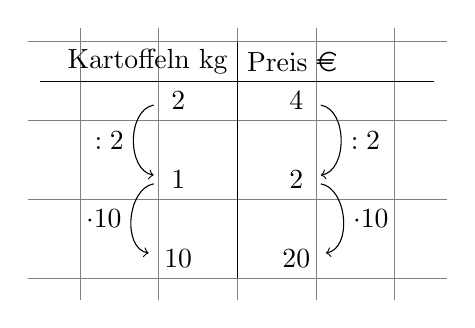
\begin{tikzpicture}[show background grid]
\draw[black] (0cm,0cm) -- (0cm,-3cm); 
\draw[black] (-2.5 cm,-0.5cm) -- (2.5cm,-0.5cm); 
\node[left] at (0 cm,-0.25cm) {Kartoffeln kg};
\node[right] at (0 cm,-0.255cm) {Preis \euro{}};
\node[circle] (1) at (-0.75 cm,-0.75cm) {2};
\node[circle] (2) at (-0.75 cm,-1.75cm) {1};
\node[circle] (3) at (-0.75 cm,-2.75cm) {10};
\node[circle] (4) at (0.75 cm,-0.75cm) {4};
\node[circle] (5) at (0.75 cm,-1.75cm) {2};
\node[circle] (6) at (0.75 cm,-2.75cm) {20};
\draw[->] (1) to [out=190,in=170] node[left] {$:2$}  (2) ;
\draw[->] (2) to [out=190,in=170] node[left] {$\cdot 10$}  (3) ;
\draw[->] (4) to [out=350,in=10] node[right] {$:2$}  (5) ;
\draw[->] (5) to [out=350,in=10] node[right] {$\cdot10$}  (6) ;
\end{tikzpicture}
&
b)&\tikzstyle{background grid}=[draw, black!15,step=.5cm]
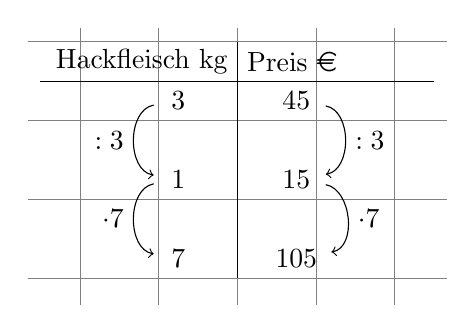
\begin{tikzpicture}[show background grid]
\draw[black] (0cm,0cm) -- (0cm,-3cm); 
\draw[black] (-2.5 cm,-0.5cm) -- (2.5cm,-0.5cm); 
\node[left] at (0 cm,-0.25cm) {Hackfleisch kg};
\node[right] at (0 cm,-0.255cm) {Preis \euro{}};
\node[circle] (1) at (-0.75 cm,-0.75cm) {3};
\node[circle] (2) at (-0.75 cm,-1.75cm) {1};
\node[circle] (3) at (-0.75 cm,-2.75cm) {7};
\node[circle] (4) at (0.75 cm,-0.75cm) {45};
\node[circle] (5) at (0.75 cm,-1.75cm) {15};
\node[circle] (6) at (0.75 cm,-2.75cm) {105};
\draw[->] (1) to [out=190,in=170] node[left] {$:3$}  (2) ;
\draw[->] (2) to [out=190,in=170] node[left] {$\cdot 7$}  (3) ;
\draw[->] (4) to [out=350,in=10] node[right] {$:3$}  (5) ;
\draw[->] (5) to [out=350,in=10] node[right] {$\cdot7$}  (6) ;
\end{tikzpicture}
\\\hline
\end{xltabular}
\vspace{0.5cm}
\end{document}